\section{Distance Measures}
\label{sec:distance}

In this section, we describe the distance measures that we use to compare attack trees. 


\begin{figure*}
    \centering
    \begin{subfigure}[b]{.40\linewidth}
        \resizebox{\linewidth}{!}{
            \begin{forest}
                for tree={
                draw,
                minimum height=.25cm,
                anchor=parent,
                align=center,
                child anchor=parent,
                edge=-
                },
                adnode/.style={rounded rectangle,},
                [{Gain Access}, adnode,
                        [{Find unlocked computer}, adnode,]
                            [{Phishing}, adnode, small angle below
                                    [{Send Email}, adnode,]
                                    [{Receive Credentials}, adnode,]]
                    ]
            \end{forest}
        }
        \caption{A simple attack tree.}
        \label{fig:dist-example-1}
    \end{subfigure}
    \begin{subfigure}[b]{.57\linewidth}
        \resizebox{\linewidth}{!}{
            \begin{forest}
                for tree={
                draw,
                minimum height=.25cm,
                anchor=parent,
                align=center,
                child anchor=parent,
                edge=-
                },
                adnode/.style={rounded rectangle,},
                [{Gain Unauthorized Access}, adnode,
                        [{Phishing}, adnode, small angle below
                                    [{Send Phishing Email}, adnode,]
                                    [{Get Credentials}, adnode,]]
                            [{Find open computer}, adnode,]
                            [{Brute force}, adnode,]
                    ]
            \end{forest}
        }
        \caption{A slightly modified attack tree.}
        \label{fig:dist-example-2}
    \end{subfigure}
    \caption{Two similar attack trees with small differences to model the distance measures.}
    \label{fig:dist-example}
\end{figure*}

% \subsection{Measurement Comparison}

% A comparison of a series of measurements of two attack trees. These measurements could include, but would not be limited to, the number of nodes, the number of leaf nodes, the number of refinements, the number of \AND\ and \OR\ refinements, the depth of the tree, and the average number of children per node. By comparing this series of measurements, we can roughly describe the difference between two attack trees. This means of measuring the difference between two trees has been used in lieu of a more established difference mechanism.

% \NS{I'm refering to myself in acceptability 1}

\subsection{Label Distance}
\label{ssec:label-distance}

Label Distance (LD) is a measure of the difference between the labels of a given tree. This is derived from the mappings suggested in Tai~\cite{tai_tree--tree_1979} and Zhang and Shasha~\cite{Zhang_Shasha_1989}, with an algorithm influenced by the A$^*$ tree edit distance algorithm from Yoshino~\etal~\cite{yoshino_dynamic_2013}. We can calculate the distance between two labels by using a pre-trained BERT model to calculate the semantic similarity between two labels. This is done by calculating the cosine similarity between the embeddings of the two labels. This is shown in Figure~\ref{fig:semanticreplacement}. We create a matrix $D$ which is an $M \times N$ matrix which represents all of the distances between the labels between two trees. We then take the largest value at index $i, j$ of this matrix and remove that row ($i$) and column ($j$) from $D$, recording the mapping between $b_i$ and $b_j$. This is repeated until all nodes are included in a mapping set. If the largest value in $D$ is below some value $\epsilon$, we consider the labels to be different, and a direct mapping is not created. We add the nodes as individuals to the mapping (mapping to/from $\Lambda$ indicating that these labels would be removed or added). We then calculate the cost of each node that would be removed or added, giving a cost of 1. This algorithm is defined in detail in Algorithm~\ref{alg:label-distance} in Appendix~\ref{appendix:alg:label-distance}. We can divide this value by the number of nodes in the largest tree to get a normalized value.



This measurement considers all the labels of each node within an attack tree. It uses a semantic comparison to examine the meanings of the nodes, which would allow for this distance measure to work on unfiltered trees. However, this measure does not consider the structure of the tree in any way, and therefore does not represent how the nodes are organized. If we examine the attack tree in Figure~\ref{fig:tartgetAT}, if create an attack tree with all the same label names, but all nodes directly attached to the root (a single root node with 13 child nodes with identical names as in Figure~\ref{fig:tartgetAT}), the resulting label distance would be zero. As such, label distance offers a way to quickly examine if the meanings of the nodes are similar, but does not offer a way to examine the structure of the tree. 


Applying LD to the examples provided in Figure~\ref{fig:dist-example}, we would first create two lists of labels of both Figures~\ref{fig:dist-example-1}~and~\ref{fig:dist-example-2}. Then we could compare these lists according to their semantic similarity along the process described in Section~\ref{sec:semantic-similarity}. The labels that are identical will be matched first, then the labels will be matched according to their semantic similarity in decreasing order. This is repeated until only the node ``brute force'' from Figure~\ref{fig:dist-example-2} remains. Provided all other nodes match (given a sufficiently permissive value of $\epsilon$), LD will result in a distance of 1 (normalized distance of 0.167).



\subsection{Tree Edit Distance}
\label{ssec:ted}

Tree edit distance is a measure of the difference between two trees by defining an optimal edit path; that is, what changes are needed to turn one tree into another. The seminal work in this field is by Zhang and Shasha~\cite{Zhang_Shasha_1989}. In their work, they describe a simple algorithm for calculating the distance between two trees. This algorithm is based on the idea of a \textit{forest} distance, which is the distance between two forests, or sets of trees. The result of this algorithm is a measure of the costs of edits needed to transform one tree into another, with the convention being that any edit requires a cost of 1. The possible edits are matching, in which two nodes are defined to be equivalent which is the only edit without cost. Insertion in which a node is added, deletion in which a node is removed, and changing one node into another, in which a node has its label replaced. We modify the Zhang and Shasha algorithm in three ways, we introduce a mechanism for comparing the semantic meaning of node labels (similar to label distance) and  a new cost for changing the refinement of a node. It is possible to take this absolute edit distance number and divide it by the tree with the largest number of nodes to find a normalized value.

The tree edit distance from Zhang and Shasha works on ordered trees, which for our purposes presents a challenge, as our attack trees are unordered. Zhang~\etal showed that unordered tree edit distance is a MAX SNP-Hard problem~\cite{zhang_max_1994}. Our assumption that attack trees do not grow to be very large allows us to remain unconcerned about the processing time of unordered tree distance. Previous work on unordered tree edit distance have offered various polynomial time approximate solutions, all making assumptions to speed up computations. Fundamentally, all make the same assumption, which is that there is absolute equivalence between nodes within two trees. Either nodes have identical labels or they do not. This would preclude their use on unfiltered data, as nodes are not guaranteed to have the same label. On unfiltered data, these algorithms may find a local maximum instead of the global maximum needed to create a mapping (as is done in label distance described in Section~\ref{ssec:label-distance}) has an issue of assuming nodes with absolute equivalence. That is, each algorithm will assume a mapping that may not be optimal if it finds two nodes to be ``equivalent'' if their similarity is above a given threshold (see Section~\ref{sssec:threshold-problem}), or it will not find a mapping between most similar nodes because these nodes do not have identical labels. As such, these algorithms are unsuitable for our purposes.


Applying TED to the examples provided in Figure~\ref{fig:dist-example}, we follow the process described in \cite{Zhang_Shasha_1989}, by calculating key roots (the rightmost parent of each subtree) and then computing forest distance. For the specific mechanics of this distance, we refer the reader to the work by Zhang and Shasha~\cite{Zhang_Shasha_1989}. The resulting distance given a reasonable value of $\epsilon$ is 5 (normalized to 0.833). This higher than for the other distance metrics as this implementation of TED is unable to handle reordered nodes.
Figures~\ref{fig:dist-example-1}~and~\ref{fig:dist-example-2}


% \subsubsection{Refinement Cost}
% One of the biggest differences between attack trees and other tree-like data structures is the presence of refinements, or the \AND\ and \OR\ relationships, which state whether all of the children of a node must be satisfied for the parent node to be satisfiable (\AND) or if at least one must be satisfied for a parent node to be satisfiable (\OR). This is a critical part of the attack tree structure and must be included in the tree edit distance algorithm.




% \begin{definition}\label{def:cost-function}
%     Similar to Zhang and Shasha, we define $\gamma$ be the cost function for the node edit distance, with the cost of removing a node to be $\gamma(\ATnode{d}{i} \rightarrow {\Lambda})$, the cost of adding a node to be $\gamma({\Lambda}\rightarrow \ATnode{d}{i})$, and the cost of changing a node to be $\gamma(\ATnode{d}{i} \rightarrow \ATnode{e}{i})$. We give the cost changing a refinement for node  $\ATnode{d}{i}$ and $\ATnode{e}{j}$ to be $\gamma(\Delta(\ATnode{d}{i}) \rightarrow \Delta(\ATnode{e}{j}))$. To simplify changing refinements, as only three refinements are given and we consider the cost of changing any refinement into another refinement to be the same, we say the cost of changing a refinement to be $\gamma(\Delta)$. That is to say $\gamma(\ATnode{d}{i} \rightarrow \ATnode{e}{j})$ for any $\ATnode{d}{i}.\Delta \ne \ATnode{e}{j}.\Delta$.
% \end{definition}


% \begin{lemma}\label{lem:gamma-delta}

%     $\gamma(\Delta)$ only applies in the case of changing one node into another.

%   \begin{proof}
%     Proof is provided in Appendix~\ref{appendix:lem:gamma-delta}
%   \end{proof}

% \end{lemma}




% \begin{lemma}\label{lem:gamma-delta-2}
%     For attack trees within the definition of Definition~\ref{def:attack-tree}. It must be the case that

%     \[\gamma(\Delta) \le \gamma(\ATnode{e}{j} \rightarrow {\Lambda}) + \gamma(\Lambda \rightarrow {\ATnode{e}{j}})\]

%     \begin{proof}
%         Proof is provided in Appendix~\ref{appendix:lem:gamma-delta-2}
%       \end{proof}

    

% \end{lemma}

% \begin{lemma}\label{lem:gamma-delta}

%     $\gamma(\Delta)$ only applies in the case of changing one node into another.

%     \begin{proof}


%         \begin{enumerate}
%             \item In the case of node removal, there can be no additional cost for changing a refinement. That is, if we remove a node $\ATnode{d}{i}$ from $T$, then we have:

%                   $$\gamma(\ATnode{d}{i} \rightarrow {\Lambda})$$

%                   $\Lambda$ is an empty tree, and by definition does not contain any refinements. Therefore, the cost of changing the refinement is zero.

%             \item In the case of adding a node, the cost of adding a refinement would be included in the cost of adding the node. That is, if we add a node $\ATnode{d}{i}$ to $T$, then we have:

%                   $$\gamma(\Lambda \rightarrow {\ATnode{d}{i}})$$

%                   It is not possible to for a node in an attack tree to not have a refinement. If we separate the cost of adding a node and the cost of adding a refinement, we have one of the two following cases:
%                   \begin{enumerate}
%                       \item A node is added without a refinement, which gives a refinement addition cost of 0, but results in an attack tree which is not valid given our attack tree definition.
%                       \item The cost of adding a refinement is \textbf{always} added to the cost of adding a node, which results in the new cost of adding a node to always include $\gamma(\Delta)$.
%                   \end{enumerate}

%                   Given one of these cases results in an invalid tree, the other case must always apply. Therefore, by convention, we do not separate the cost of adding a node and the cost of adding a refinement, these are one and the same.

%             \item In the case of replacing a node, the cost of replacing a refinement would be:

%                   $$\gamma({\ATnode{d}{i}} \rightarrow {\ATnode{e}{j}})$$

%                   Which we declare to consist of the sum following two costs:

%                   $$\gamma({\ATlabel{d}{i}} \rightarrow {\ATlabel{e}{j}})$$

%                   Which is the cost of changing one label to another. This is the original cost of replacing a node according to Zhang-Shasha. We also have:

%                   $$\gamma(\Delta)$$

%                   Which as previously stated is the cost of changing a refinement.



%         \end{enumerate}

%     \end{proof}

% \end{lemma}




% \begin{lemma}\label{lem:gamma-delta-2}
%     For attack trees within the definition of Definition~\ref{def:attack-tree}. It must be the case that

%     \[\gamma(\Delta) \le \gamma(\ATnode{e}{j} \rightarrow {\Lambda}) + \gamma(\Lambda \rightarrow {\ATnode{e}{j}})\]

%     \begin{proof}
%         Let $T$ be an attack tree.

%         Assume that $\gamma(\Delta) > \gamma(\ATnode{e}{j} \rightarrow {\Lambda}) + \gamma(\Lambda \rightarrow {\ATnode{e}{j}})$.

%         Let $S$ be the optimal sequence of edit operations according to the Zhang-Shasha algorithm. That is, $\gamma(S)$ is minimal for all possible edit sequences for $\delta(T_1, T_2)$ Let some operation $s \in S$ be an operation to replace some node, $\ATnode{d}{i}$, with another, $\ATnode{e}{j}$.

%         Thus, $\gamma(s) = \gamma({\ATlabel{d}{i}} \rightarrow {\ATlabel{e}{j}}) + \gamma(\Delta)$

%         We have two cases:

%         \begin{enumerate}
%             \item $\ATnode{d}{i}.\Delta = \ATnode{e}{j}.\Delta$

%                   In this case, both $\ATnode{d}{i}$ and $\ATnode{e}{j}$ have the same refinement. Thus, $\gamma(\Delta) = 0$. Therefore, $\gamma(s) = \gamma({\ATlabel{d}{i}} \rightarrow {\ATlabel{e}{j}})$.

%             \item $\ATnode{d}{i}.\Delta \ne \ATnode{e}{j}.\Delta$

%                   In this case, both $\ATnode{d}{i}$ and $\ATnode{e}{j}$ have different refinements. Thus, $\gamma(\Delta) > 0$. Therefore, $\gamma(s) = \gamma({\ATlabel{d}{i}} \rightarrow {\ATlabel{e}{j}}) + \gamma(\Delta)$.

%                   However, we have assumed that $\gamma(\Delta) > \gamma(\ATnode{e}{j} \rightarrow {\Lambda}) + \gamma(\Lambda \rightarrow {\ATnode{e}{j}})$. Therefore, $\gamma(s) = \gamma({\ATlabel{d}{i}} \rightarrow {\ATlabel{e}{j}}) + \gamma(\Delta) > \gamma(\ATnode{e}{j} \rightarrow {\Lambda}) + \gamma(\Lambda \rightarrow {\ATnode{e}{j}})$, as by convention $\gamma$ cannot result in a negative value.

%                   As such, we can replace $s$ with the sequence of operations $s_1$ and $s_2$, where $s_1$ is the operation to remove $\ATnode{d}{i}$ and $s_2$ is the operation to add $\ATnode{e}{j}$. Thus, $\gamma(s_1) = \gamma(\ATnode{e}{j} \rightarrow {\Lambda})$ and $\gamma(s_2) = \gamma(\Lambda \rightarrow {\ATnode{e}{j}})$. Therefore, $\gamma(s_1) + \gamma(s_2) < \gamma(s)$.

%                   This results in a contradiction, as $S$ is the optimal sequence of edit operations according to the Zhang-Shasha algorithm, it must not be possible to replace any $s \in S$ with an operation, or sequence of operations, with lower cost.
%         \end{enumerate}

%         Therefore, if $\gamma(\Delta) > \gamma(\ATnode{e}{j} \rightarrow {\Lambda}) + \gamma(\Lambda \rightarrow {\ATnode{e}{j}})$, then $\gamma(\Delta)$ either must be 0 for a change node edit operation to be included in the optimal sequence of edit operations (case 1), or the optimal sequence of edit operations must always result in node removal then replacement (case 2). In both cases, $\gamma(\Delta)$ is not used.

%         Therefore, in order to include the cost of changing refinements in the cost of replacing a node, it must be the case that $\gamma(\Delta) \le \gamma(\ATnode{e}{j} \rightarrow {\Lambda}) + \gamma(\Lambda \rightarrow {\ATnode{e}{j}})$.


%     \end{proof}


% \end{lemma}



% As the cost of replacing refinements is ever present, we can simply apply the cost of the replacing refinements after computing the tree edit distance by following the mappings and subsequently applying changed refinements. By doing this, we do not add to the time complexity of the Zhang and Shasha algorithm.

% This method of computation works as it is not possible to have an intermediate attack tree node without a refinement~\cite{mauw_foundations_2006}. As such, all non-leaf nodes are either \AND\ or \OR\ nodes, so the distance between refinements is simple given as the cost needed to convert from one refinement to the other. As unlike the calculations of adding ($\Lambda \rightarrow i$), removing ($i \rightarrow \Lambda$), or replacement ($i \rightarrow j$), with refinements there is only on possible operation: replacement: either \AND $\rightarrow$ \OR\ or \OR $\rightarrow$ \AND.



% \subsubsection{Children Reordering}
% The Zhang and Shasha edit distance algorithm is specifically given for ordered trees, that is, the order of child nodes is taken to be significant. In attack trees without sequential conjunction, the order of nodes is not given to be significant~\cite{mauw_foundations_2006,jhawar_attack_2015}. This results in an issue where trees with identical, but unordered nodes are given to have a high edit distance. This is shown in Figure~\ref{fig:nodeflipping}, where two trees with identical information but different node order are given to have a distance of 2. This is due to the fact that the Zhang and Shasha algorithm is not designed to handle unordered trees. Zhang and Jiang have shown that the tree edit distance problem for unordered trees is an MAX SNP-hard~\cite{zhangMAXSNPhardResults1994}. We suggest a novel method for handling tree edit distance in unordered attack trees by taking advantage of the inherent structure of attack trees.


% \begin{figure}
%     \begin{subfigure}{.45\linewidth}
%         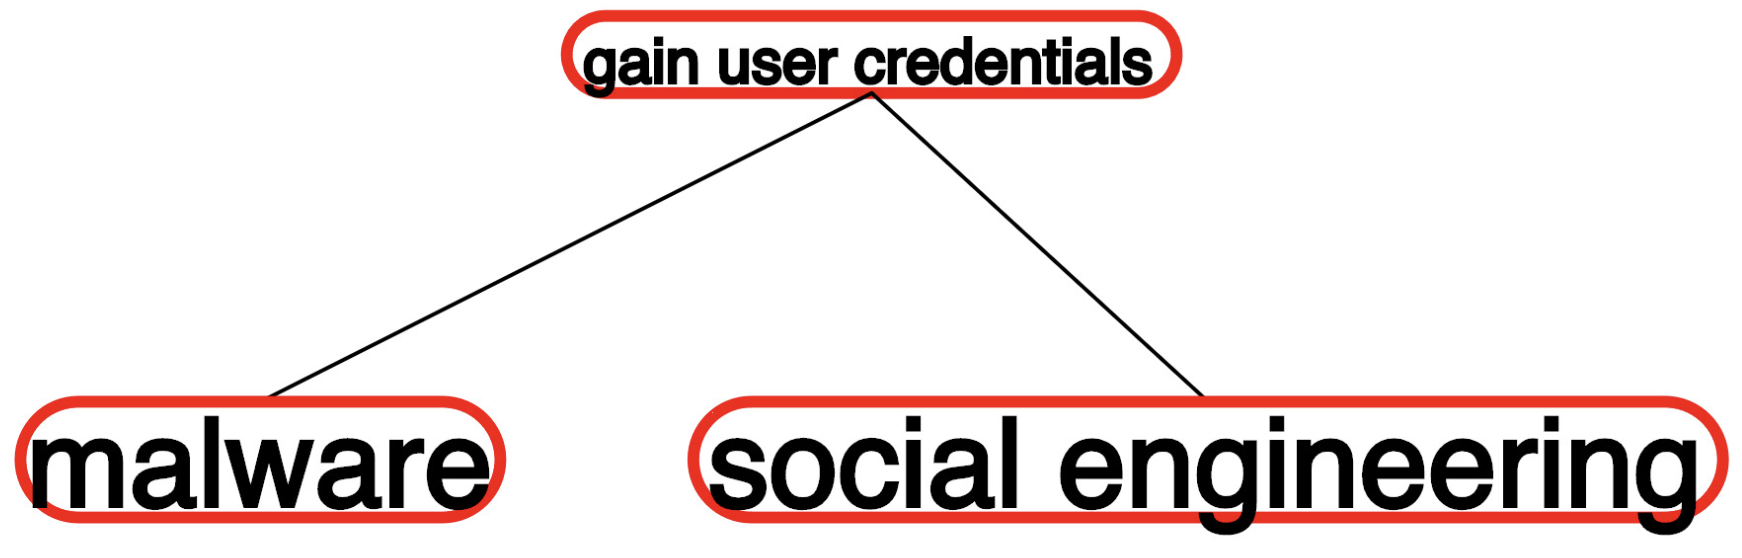
\includegraphics[width=\linewidth]{img/NodeFlip1.png}
%     \end{subfigure}
%     \begin{subfigure}{.45\linewidth}
%         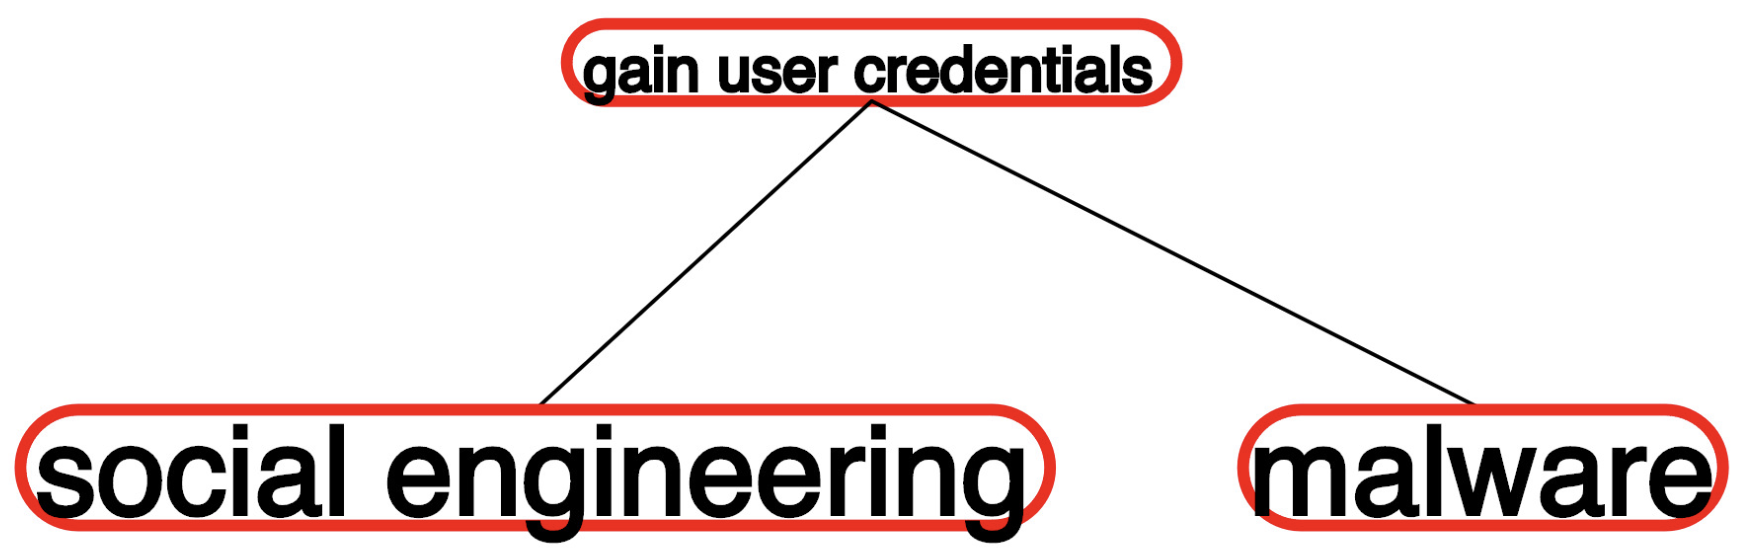
\includegraphics[width=\linewidth]{img/NodeFlip2.png}
%     \end{subfigure}
%     \caption{Two attack trees (subtrees of the example in Figure~\ref{fig:tartgetAT}) with identical information but different node order. These trees would evaluate to have a distance of 2 (two replacement operations).}
%     \label{fig:nodeflipping}
% \end{figure}

% Attack trees, by virtue of their construction, tend to be organized in levels of abstraction. That is, with each new level of an attack tree, the nodes are given to be more specific than the nodes in the previous level. This is shown in Figure~\ref{fig:tartgetAT}, where the root node is given to be the most abstract (as the overall goal), while the leaf nodes are the most concrete (as the individual actions). From this, we find siblings in an attack tree to be on the same level of abstraction. As such, the order of siblings can be changed without affecting the meaning of the attack tree. By checking the order of sibling sets between the two attack trees



% \begin{algorithm}
%     \caption{An algorithm to reorder siblings based on semantic similarity}
%     \label{alg:sibling_reorder}
%     \begin{algorithmic}
%         \State Two attack trees $T_1$ and $T_2$ according to Definition~\ref{def:attack-tree} with $a$ and $b$ total nodes respectively
%         \State $M$ is the mapping of nodes between $T_1$ and $T_2$ \Comment{We give $m[0]$ and $m[1]$ to be the source and target nodes of a mapping for $m \in M$}
%         \State $M \gets T_1[a]\mapsto T_2[b]$\Comment{Root nodes are always mapped}
%         \For{$m \in M$}

%         \State $D \gets []$ \Comment{Matrix of semantic similarity values}
%         \For{left-wise index $i$ in $m[0].\text{children}$}
%         \For{leftwise index $j$ in $m[1].\text{children}$}
%         \State $D[i][j] \gets$
%         \State$\text{  }\text{  }\text{  }\text{  }\text{  }\text{  }\text{  }\text{  }\text{  }\delta(m[0].\text{children}[i].\text{label}, m[1].\text{children}[j].\text{label})$
%         \EndFor
%         \EndFor
%         \State $M_t \gets \emptyset$ \Comment{Temporary set of mappings}
%         \While{$D$ is not empty}
%         \State $i, j \gets \text{argmax}(D)$ \Comment{Largest value in $D$}
%         \State $M_t \gets M_t \cup m[0].\text{children}[i]\mapsto m[1].\text{children}[j]$
%         \State $D \gets D - i$ \Comment{Remove row $i$}
%         \State $D \gets D - j$ \Comment{Remove column $j$}
%         \EndWhile
%         \For{$p$ in $M_t$}
%         \If{indicies $i$, $j$ of $p$ are not equal}
%         \State{Swap nodes $i$ and $j$ \textbf{in $T_1$}}
%         \EndIf
%         \EndFor
%         \State $M \gets M \cup M_t$
%         \EndFor
%     \end{algorithmic}
% \end{algorithm}




\subsection{Radical Distance (RD)}
\label{ssec:rd}

In a previous work on attack trees, a proposed mechanism of attack tree decomposition focused on the concept of radicals, or subtrees consisting of a single parent, refinement, and set of children~\cite{schiele2021novel}. We take this decomposition and compare the resulting set of radicals. We define the distance between the resulting radicals according to Algorithm~\ref{alg:recursive-radical} in Appendix~\ref{appendix:alg:radical-distance}.

In Radical Distance (RD), we first decompose into a collection of subtrees that are each a single height, indexed by each subtree's root node. We then perform a semantic comparison of each of the subtree roots, finding a semantic mapping similar to the one discussed for label distance in Section~\ref{ssec:label-distance}. We then calculate the distance subtree by subtree, adding a distance of 1 if the root nodes are not equal, a distance of 0.5 if the refinements are not equal. For the children, we perform an operation very similar to label distance, but we do not add distance to our calculation if one of the children is already present as a key of the radical dictionaries, as this would result in double counting of that child. This repeats until all children are compared, added or removed.

RRD as we have defined it does not contain a mechanism to enable tracking of modifications unlike tree edit distance. Unlike label distance however, the full structure of the tree is taken into account. Just as almost all distances we have proposed, our distance does account for the semantic difference between node labels.

Applying RD to the examples provided in Figure~\ref{fig:dist-example}, we first compute the radical decomposition of both attack trees. These are the one height subtrees rooted at ``Gain Access'' and ``Phishing'' for Figure~\ref{fig:dist-example-1} and ``Gain Unauthorized Access'' and ``Phishing'' for Figure~\ref{fig:dist-example-2}. We then compute the semantic distance between the root nodes of each of the radicals, in a manner similar to LD, taking the most closely related radicals first. In this case, the two radical roots that are identical (``Phishing'') are selected first, and the radical distance is calculated by comparing the root nodes, refinements, and all children (excluding children that themselves are roots of other radicals). In this case, this comparison yields a difference of 0 given a reasonable value of $\epsilon$. This is repeated for the other two radicals, which have a distance of 1 (``brute force''), resulting in an overall distance of 1 (normalized to 0.167).


\subsection{Multiset Difference (MSD)}
\label{ssec:msd}

Attack trees can be represented mathematically in many different ways. The definition we offer in Definition~\ref{def:attack-tree} is a recursive definition. Multiple different representations of attack trees have been proposed, the arguably most established attack tree semantics would be multiset semantics proposed by Mauw and Oostdijk~\cite{mauw_foundations_2006}. In multiset semantics, each multiset represents a single a complete attack vector within the attack tree. A multiset consisting of multisets represents a node with multiple children. For defining multiset difference, we can use the Jaccard distance between two multisets. However, if we were to use this method, we would need node labels in order for the elements to be considered identical.

If we want to expand the Jaccard distance to count similar meaning elements of multisets as identical, we would need to calculate the semantic similarity between the elements of the multisets. This would result in a similar problem to the label distance problem or the modification of Zhang and Shasha tree edit distance, as we would need to define a threshold $\epsilon$ for the semantic similarity between two elements. This would result in the same threshold problem as described in Section~\ref{sssec:threshold-problem}, but allow for the multiset distance to account for similar meaning but not identical labels.

Multiset semantics, like most mathematical attack tree semantics, contain only the leaf node labels. All other labels are reduced from the tree. Additionally, the exact structure of the tree is not generally reconstructible. Ultimately, semantics are means to answer the question of if two trees are equivalent, which would mean that the exact structure of tree is not necessarily important. In tree distance, however, the exact structure may be important. By comparing the difference between multisets, we lose some information about the structure of the tree. We also lose the information contained in any intermediate nodes within the tree.

Applying MSD to the examples provided in Figure~\ref{fig:dist-example}, we first calculate the multiset semantic representations of both trees. These semantics would be $\{\{\text{Send Email},$ $\text{Recieve Credentials},\},$ $\{\text{Find unlocked computer}\}\}$ for Figure~\ref{fig:dist-example-1} and $\{\{\text{Send Phishing Email}, \text{Get Credentials}\},$ $\{\text{Find open computer}\},$ $\{\text{Brute force}\}\}$ for Figure~\ref{fig:dist-example-2}. We then calculate the Jaccard distance between each possible pair of set, using semantic similarity to determine equivalence of the elements in each set. Starting from the pair of sets with the lowest jaccard distance (the sets $\{\text{Find unlocked computer}\}$ and $\{\text{Find open computer}\}$), we add the Jaccard distance of these sets (in this case 0) to the overall distance measure. These sets are then removed from the list of sets. This is repeated until all sets are compared, and any sets remaining (in this case $\{\text{Brute force}\}$) are compared to an empty set. In this case, this yields a a distance of 1 (normalized to be 0.167) for a reasonable value of $\epsilon$.



\subsection{Weighted Sum Distance (WSD)}
\label{ssec:wsd}

This is a weighted average of the above distance values. We will validate and asses the four distance measures described in this section according to our experimental design described in Section~\ref{sec:methodology}. We will then attempt to propose a single distance measure that is the weighted sum of the other four distance measures. This weighted sum can be expressed as the following:
\[
    \alpha_1*\text{LD}+ \alpha_2*\text{TED} + \alpha_3*\text{RD} + \alpha_4*\text{MSD}
\]

For a given vector $\alpha = [\alpha_1, \alpha_2, \alpha_3, \alpha_4]$. We will attempt to provide an optimal alpha such that the performance of this weighted sum outperforms any individual distance measure shown above.

Applying WSD to the examples provided in Figure~\ref{fig:dist-example}, we would first calculate LD, TED, RD, and MSD for the two trees. We would then calculate the weighted sum of these values according to the selected value of $\alpha$ to find the WSD. The value of WSD will depend both on the value of $\epsilon$ (as it will affect the four primary distance measures) as well as the selected values of $\alpha$, which affect the sum.

% \subsection{Tree Embedding Distance}

% \NS{I can't find a good way to do this - I could simulate this by combinding BFS position data with the label semantic embeddings, but I dunno if this is a good option}
% Algorithm 2 An algorithm to reorder siblings based on semantic
% similarity


